
\chapter{Results}
\label{ch:results}

This chapter presents the outcomes of our experiments designed to assess the model's performance under various configurations and data conditions relevant to clinical settings. We evaluate the model's robustness to class imbalance, the impact of different normalization techniques, and its resilience to noise, with a particular focus on how these factors affect predictive accuracy and calibration.

We begin by comparing baseline models to validate our implementation and ensure alignment with previously published results. Subsequently, we assess the impact of class rebalancing and gradient clipping on the model's calibration and probability estimates, helping identify optimal configurations for model stability and accurate probability predictions. Next, we explore the effects of \gls{ecdf} normalization compared to Z-score normalization in terms of value forecasting and mortality prediction. This examination reveals the benefits and trade-offs associated with each normalization method. Finally, we evaluate the model's resilience to Gaussian and uniform noise. By comparing performance metrics under different noise conditions, we assess how each normalization method performs in the presence of outliers and noise typical for clinical data.

Throughout this chapter, results are reported as averages over 10 runs with standard errors of the mean (\( \text{Mean} \pm \text{SE} \)). In the tables, the relative differences from the baseline, indicated by the underlined text, is provided as the signed percentage change. The percentage change is calculated as follows: $\frac{X - X_{baseline}}{X_{baseline}} \times 100\%$, where $X$ is the performance metric of the given experiment and $X_{baseline}$ is the performance metric of the baseline. Arrows (\textuparrow~ and \textdownarrow) are used to indicate the desired direction of change for each metric (``higher is better'' and ``lower is better'' respectively). Figures illustrate average performance with error bands representing the standard error of the mean.


\section{Baseline models comparison}
\label{sec:baseline_models_comparison}

As shown in \cref{fig:baseline_results}, the \citefield{STraTS2022}{shorttitle} model exhibits superior performance over other baselines, which is consistent with the original paper results. Additionally, our implementation achieves comparable and even slightly improved predictive performance (up to \qty{5}{\percent} higher on \gls{aucpr}) across all data fractions, indicating that our modifications did not compromise the predictive capabilities of the model.


\begin{table}
\begin{tabular}{p{1.5cm}lccc}
\toprule
Data fraction &   & ROC-AUC \textuparrow & AUC-PR \textuparrow & min(Re,Pr) \textuparrow   \\
\midrule
\multirow[t]{6}{*}{10\%} & \underline{STraTS} & 0.878\(\pm\)0.001 & 0.532\(\pm\)0.002 & 0.515\(\pm\)0.004 \\
 & GRU & 0.855\(\pm\)0.002 \(-3\%\) & 0.476\(\pm\)0.005 \(-11\%\) & 0.473\(\pm\)0.002 \(-8\%\) \\
 & SAND & 0.844\(\pm\)0.004 \(-4\%\) & 0.463\(\pm\)0.008 \(-13\%\) & 0.462\(\pm\)0.006 \(-10\%\) \\
 & GRU-D & 0.860\(\pm\)0.003 \(-2\%\) & 0.484\(\pm\)0.006 \(-9\%\) & 0.482\(\pm\)0.006 \(-6\%\) \\
 & TCN & 0.838\(\pm\)0.007 \(-5\%\) & 0.446\(\pm\)0.011 \(-16\%\) & 0.458\(\pm\)0.007 \(-11\%\) \\
 & Ours & \textbf{0.884\(\pm\)0.001 \(+1\%\)} & \textbf{0.556\(\pm\)0.003 \(+5\%\)} & \textbf{0.530\(\pm\)0.002 \(+3\%\)} \\
\cline{1-5}
\multirow[t]{6}{*}{50\%} & \underline{STraTS} & 0.891\(\pm\)0.000 & 0.571\(\pm\)0.002 & 0.539\(\pm\)0.002 \\
 & GRU & 0.880\(\pm\)0.002 \(-1\%\) & 0.543\(\pm\)0.004 \(-5\%\) & 0.519\(\pm\)0.003 \(-4\%\) \\
 & SAND & 0.873\(\pm\)0.002 \(-2\%\) & 0.525\(\pm\)0.004 \(-8\%\) & 0.510\(\pm\)0.003 \(-5\%\) \\
 & GRU-D & 0.885\(\pm\)0.002 \(-1\%\) & 0.548\(\pm\)0.004 \(-4\%\) & 0.530\(\pm\)0.004 \(-2\%\) \\
 & TCN & 0.869\(\pm\)0.002 \(-2\%\) & 0.515\(\pm\)0.004 \(-10\%\) & 0.506\(\pm\)0.003 \(-6\%\) \\
 & Ours & \textbf{0.898\(\pm\)0.000 \(+1\%\)} & \textbf{0.596\(\pm\)0.001 \(+4\%\)} & \textbf{0.553\(\pm\)0.001 \(+3\%\)} \\
\cline{1-5}
\multirow[t]{6}{*}{100\%} & \underline{STraTS} & 0.896\(\pm\)0.000 & 0.589\(\pm\)0.001 & \textbf{0.554\(\pm\)0.001} \\
 & GRU & 0.886\(\pm\)0.001 \(-1\%\) & 0.558\(\pm\)0.002 \(-5\%\) & 0.532\(\pm\)0.002 \(-4\%\) \\
 & SAND & 0.879\(\pm\)0.000 \(-2\%\) & 0.548\(\pm\)0.002 \(-7\%\) & 0.527\(\pm\)0.002 \(-5\%\) \\
 & GRU-D & 0.889\(\pm\)0.001 \(-1\%\) & 0.567\(\pm\)0.002 \(-4\%\) & 0.540\(\pm\)0.002 \(-3\%\) \\
 & TCN & 0.876\(\pm\)0.001 \(-2\%\) & 0.535\(\pm\)0.002 \(-9\%\) & 0.524\(\pm\)0.003 \(-5\%\) \\
 & Ours & \textbf{0.898\(\pm\)0.000 \(+0\%\)} & \textbf{0.599\(\pm\)0.001 \(+2\%\)} & 0.553\(\pm\)0.001 \(-0\%\) \\
\cline{1-5}
\bottomrule
\end{tabular}

\caption{Coparison of baseline models on mortality prediction performance for different percentages of labeled data averaged over 10 runs.}
\label{tab:baseline_experiments}
\end{table}


\begin{figure}
    \centering
    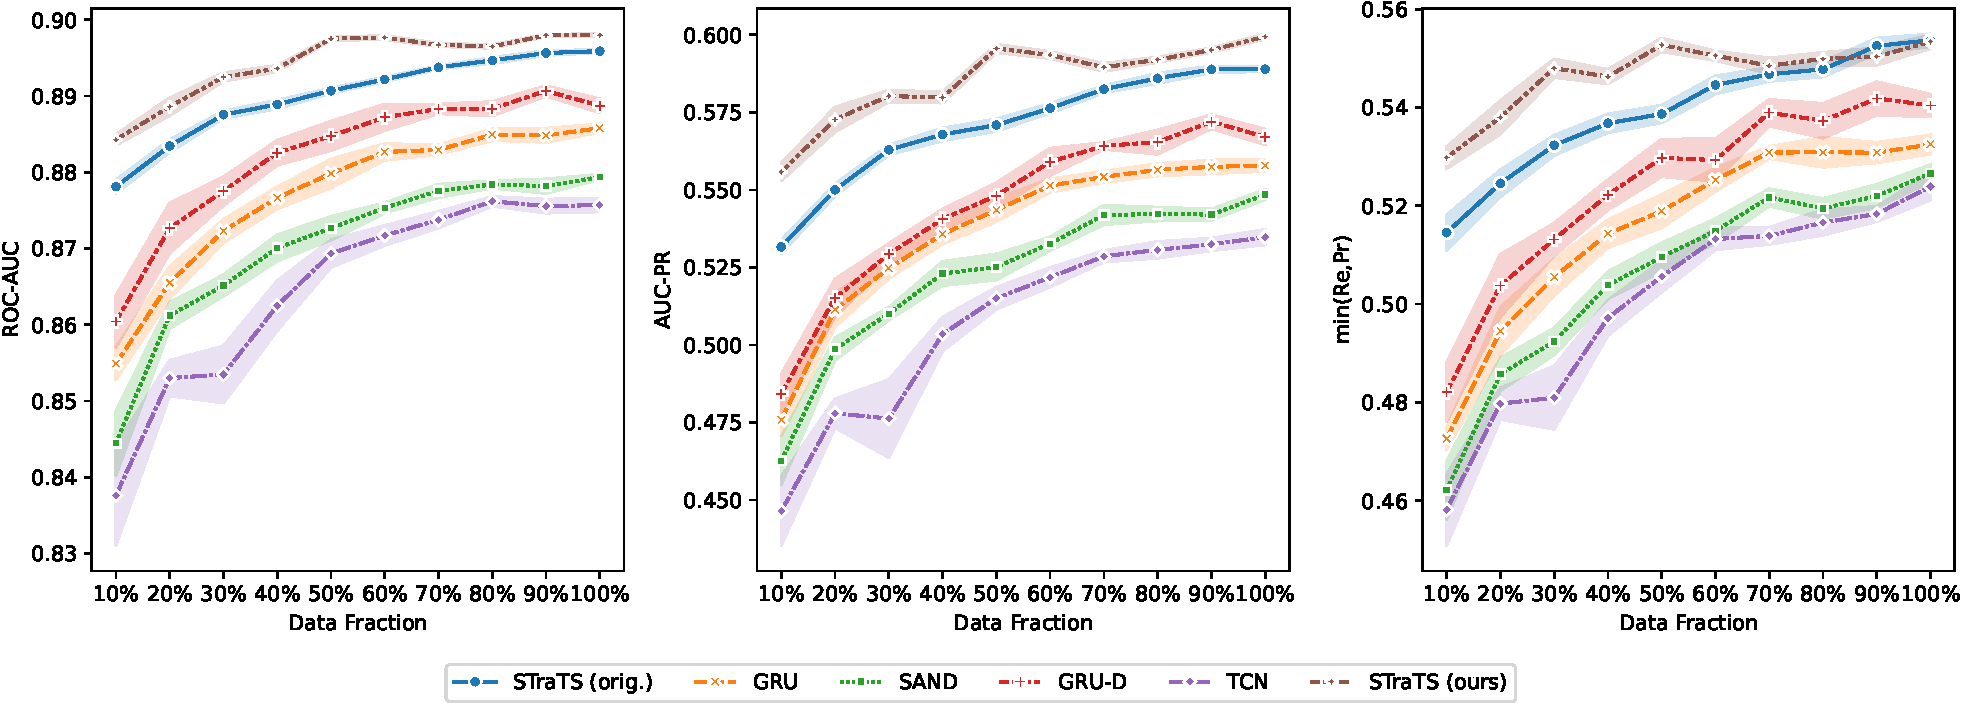
\includegraphics[width=\textwidth]{./figures/baseline_results}
    \caption{Mortality prediction performance of selected baseline models for different percentages of labeled data.}
    \label{fig:baseline_results}
\end{figure}


\section{Performance gains}

\label{sec:performance_gains}
%The  improvements mentioned in \cref{sec:implementation_details} allowed to significantly speedup the training process of the model, reducing the training time from \qty{24.081882(2.171039)}{\minute} and \qty{75.794389(3.999913)}{\minute} to \qty{0.812009(0.11482)}{\minute} and \qty{3.142936(0.25763)}{\minute} for 0.1 and 0.5 training data fractions, respectively compared to the original implementation taken from paper's GitHub. Thit is a speedup of \num{29.65716144}x and \num{24.11579141}x, respectively, compared to the original implementation.

The improvements mentioned in \cref{sec:implementation_details} allowed to significantly speedup the training process of the model, reducing the training time from \qty{24(2)}{\minute} and \qty{76(4)}{\minute} to \qty{0.8(0.1)}{\minute} and \qty{3(0.3)}{\minute} for \qty{10}{\percent} and \qty{50}{\percent} training data fractions, respectively compared to the original implementation taken from paper's GitHub. This is a speedup of \num{30}x and \num{24}x, respectively, compared to the original implementation.



\section{Results 1: Impact of Class Rebalancing and Gradient Clipping}

In addition to the previously used metrics, we estimated the mean predicted mortality risc score and compared it to the true mortality rate in the test dataset (\num{\SupervisedTestDeathPrevalence}), as described in \cref{eq:mre}. The results are presented in \cref{tab:experiment_balancing}, under the Mean Relative Error (MRE) column.

\begin{table}[h]
    \centering
    \begin{tabular}{p{1.5cm}lcccc}
\toprule
Data fraction &   & ROC-AUC \textuparrow & AUC-PR \textuparrow & min(Re,Pr) \textuparrow & MRE \textbar \textdownarrow \textbar   \\
\midrule
\multirow[t]{5}{*}{10\%} & $\beta_{16}$ & \textbf{0.885\(\pm\)0.001} & 0.553\(\pm\)0.003 & 0.529\(\pm\)0.003 & -17.3\% \\
 & $\beta_{16} + os$ & 0.884\(\pm\)0.001 & 0.544\(\pm\)0.005 & 0.524\(\pm\)0.004 & +150.5\% \\
 & $\beta_{16} + w + c$ & 0.884\(\pm\)0.001 & 0.556\(\pm\)0.003 & \textbf{0.530\(\pm\)0.002} & -21.0\% \\
 & $\beta_{4} + w + c$ & 0.875\(\pm\)0.002 & 0.549\(\pm\)0.002 & 0.524\(\pm\)0.003 & -59.5\% \\
 & $\beta_{4} + w$ & \textbf{0.885\(\pm\)0.001} & \textbf{0.559\(\pm\)0.004} & 0.527\(\pm\)0.004 & \textbf{-13.1\%} \\
\cline{1-6}
\multirow[t]{5}{*}{50\%} & $\beta_{16}$ & 0.895\(\pm\)0.000 & 0.584\(\pm\)0.002 & 0.546\(\pm\)0.002 & -16.7\% \\
 & $\beta_{16} + os$ & 0.895\(\pm\)0.000 & 0.580\(\pm\)0.002 & 0.549\(\pm\)0.002 & +140.0\% \\
 & $\beta_{16} + w + c$ & \textbf{0.898\(\pm\)0.000} & \textbf{0.596\(\pm\)0.001} & \textbf{0.553\(\pm\)0.001} & -16.1\% \\
 & $\beta_{4} + w + c$ & 0.893\(\pm\)0.000 & 0.586\(\pm\)0.001 & 0.549\(\pm\)0.002 & -55.5\% \\
 & $\beta_{4} + w$ & 0.895\(\pm\)0.001 & 0.585\(\pm\)0.002 & 0.546\(\pm\)0.001 & \textbf{-11.1\%} \\
\cline{1-6}
\multirow[t]{5}{*}{100\%} & $\beta_{16}$ & \textbf{0.899\(\pm\)0.000} & 0.597\(\pm\)0.001 & 0.551\(\pm\)0.002 & \textbf{-11.5\%} \\
 & $\beta_{16} + os$ & 0.898\(\pm\)0.000 & 0.593\(\pm\)0.001 & 0.548\(\pm\)0.002 & +137.9\% \\
 & $\beta_{16} + w + c$ & 0.898\(\pm\)0.000 & \textbf{0.599\(\pm\)0.001} & \textbf{0.553\(\pm\)0.001} & -20.4\% \\
 & $\beta_{4} + w + c$ & 0.894\(\pm\)0.000 & 0.595\(\pm\)0.001 & 0.548\(\pm\)0.001 & -58.1\% \\
 & $\beta_{4} + w$ & \textbf{0.899\(\pm\)0.000} & 0.597\(\pm\)0.001 & 0.552\(\pm\)0.002 & -11.8\% \\
\cline{1-6}
\bottomrule
\end{tabular}

    \caption{Performance metrics for different class balancing strategies. \\
    Notations are as follows: \emph{w} indicates \gls{wbce} loss; \emph{c} indicates gradient clipping; $\beta_{4}$ and $\beta_{16}$ denote batch sizes; \emph{os} indicates oversampling to achieve class balance.
    }
    \label{tab:experiment_balancing}
\end{table}

To further explore the cause of the discrepancy between the predicted and actual positive class probabilities, we inspected the distribution of predicted risk scores for the positive and negative classes as shown in \cref{fig:risk_score_distributions}.

In the experiment with class rebalancing ($\beta_{16}+os$), the average predicted probability of the positive class is more than two times higher than the true mortality rate. This effect is more pronounced with smaller data fractions, reaching MRE of \qty{+150}{\percent}, and slightly decreasing to \qty{+138}{\percent} with larger amounts of data. Further analysis of the predicted risk score distributions shows that the $\beta_{16}+os$ experiment demonstrates the best separation between the positive and negative classes; however, it is also the most biased towards predicting the positive class for observations that actually belong to the negative class. As can be seen in the upper right plot of \cref{fig:risk_score_distributions}, the area of high (\( \hat{y} > 0.5 \)) risk scores is dominated by samples from negative class, indicating that the model often predicts high risk scores for this population.

Using a smaller batch size with gradient clipping (experiment $\beta_{4} + w + c$) results in the average predicted probability of the positive class being significantly lower than the true mortality rate (MRE from \qtyrange{-59}{-55}{\percent}). Across all reported data fractions, the average predicted risk score is more than twice as small as the actual prevalence, indicating that the model underestimates the risk. As shown in \cref{fig:risk_score_distributions}, the model tends to predict risk scores clustered near 0 and 1, suggesting high confidence in its predictions. However, a majority of the positive class predictions are concentrated around 0, leading to overly confident negative predictions for mortality. Meanwhile, the experiment without gradient clipping (experiment $\beta_{4} + w$) does not exhibit the same behavior as the model with gradient clipping under small batch sizes.

\begin{figure}
    \centering
    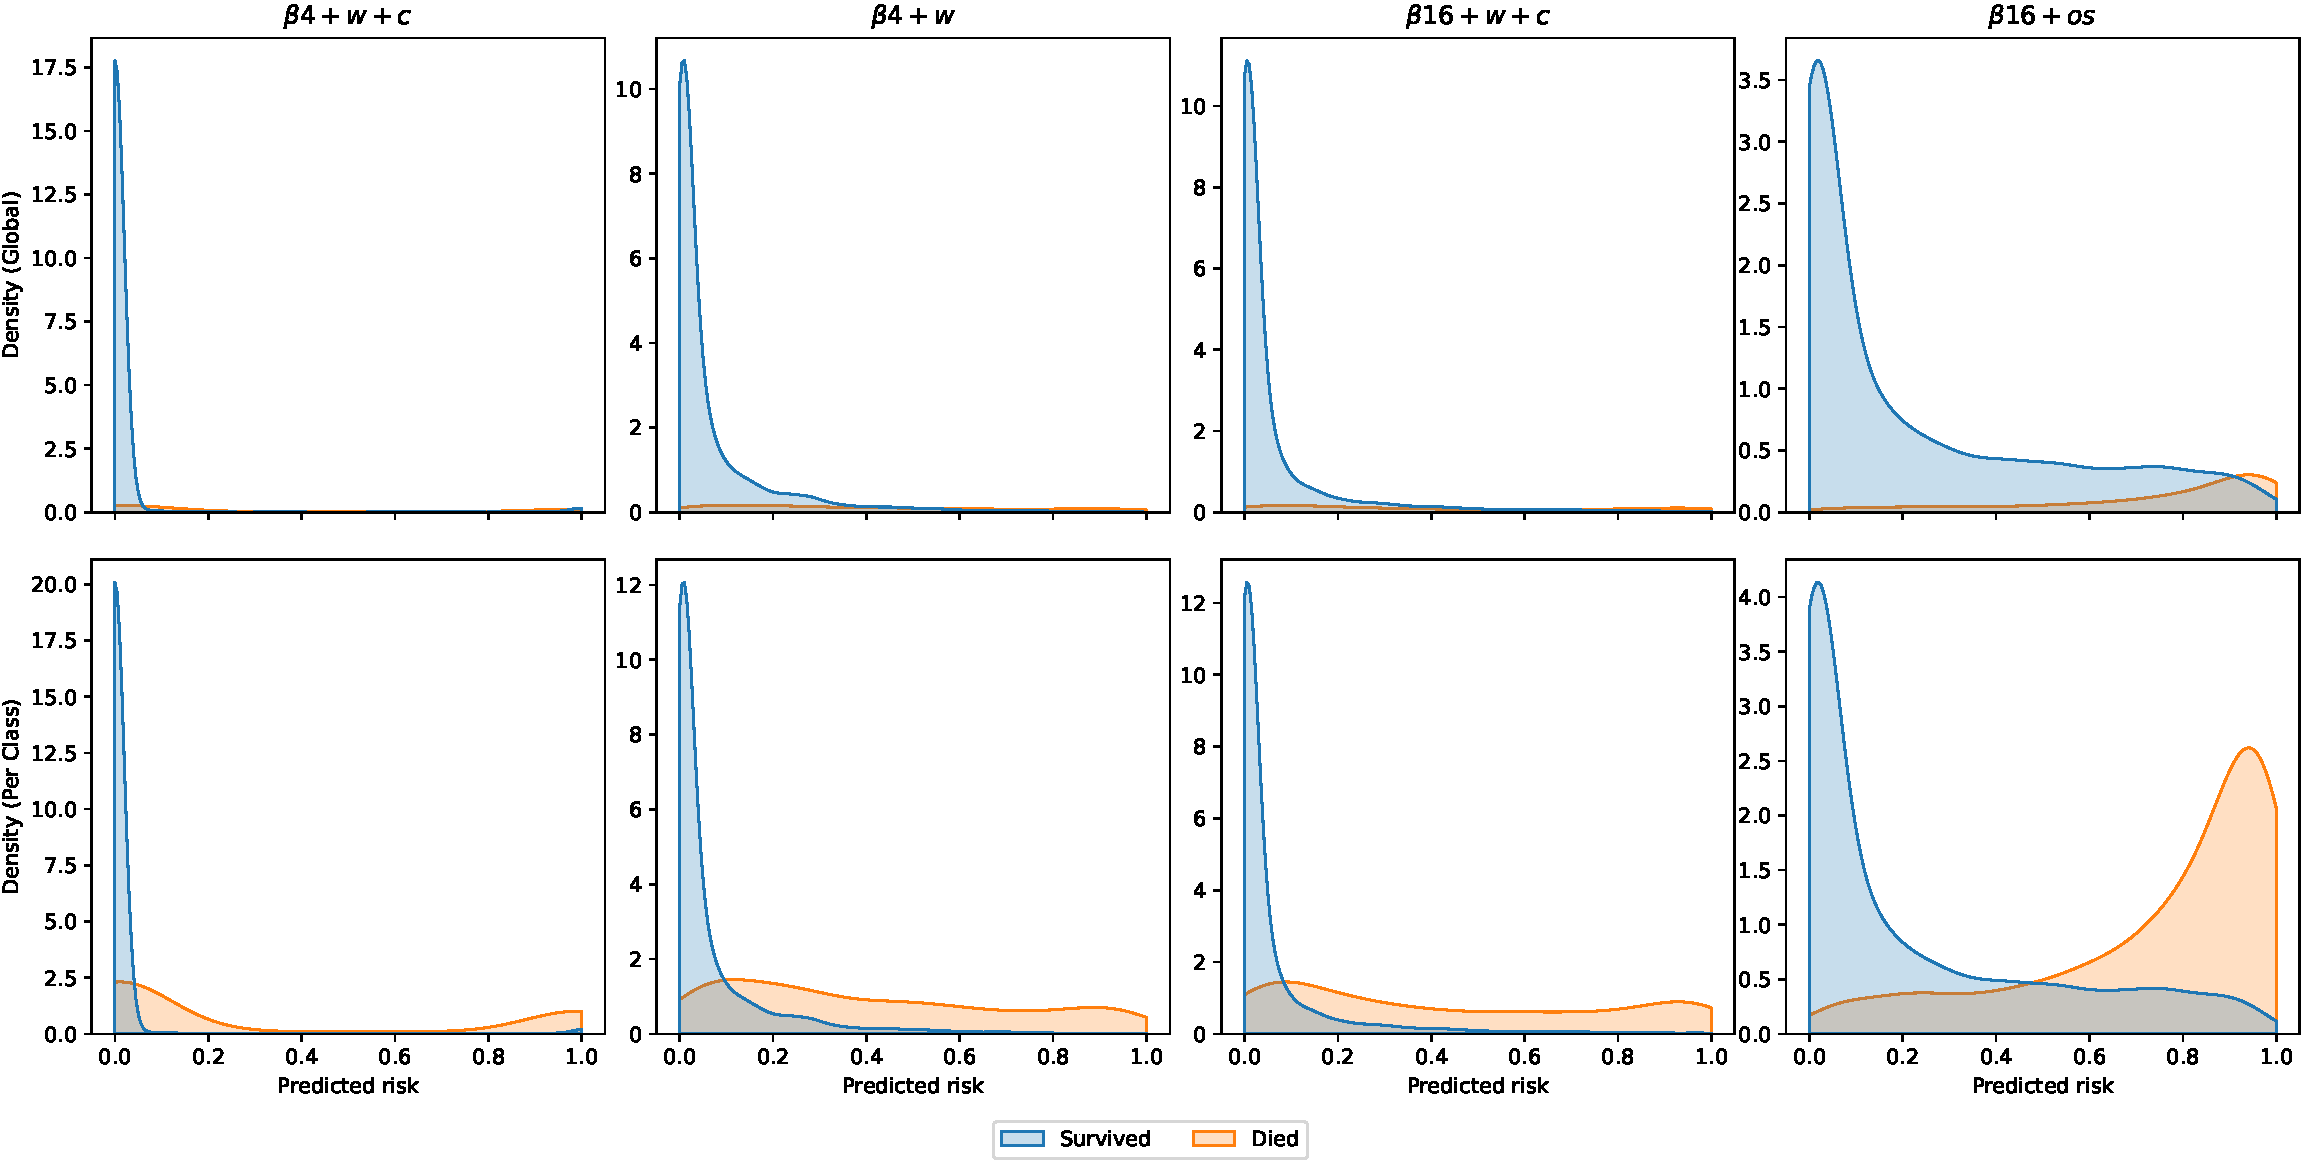
\includegraphics[width=\textwidth]{./figures/risk_score_distributions}
    \caption{Distribution of predicted risk scores for the positive and negative classes.
    In the upper row the combined area under both curves is normalized to 1, highlighting the relative frequency of predictions for each class.
    In the lower row the area under each curve is normalized to 1, allowing comparison of the probability density functions for each class independently. \\
    Notations are as follows: \emph{w} indicates \gls{wbce} loss; \emph{c} indicates gradient clipping; $\beta_{4}$ and $\beta_{16}$ denote batch sizes; \emph{os} indicates oversampling to achieve class balance.}
    \label{fig:risk_score_distributions}
\end{figure}

\paragraph{Considerations for the following experiments}

This analysis indicates that a batch size of \(16\) is sufficient for maintaining robust model performance, achieving the highest \gls{minrp} across all data fractions while consistently maintaining high \gls{auroc} and \gls{aucpr}. Class rebalancing, while useful, risks overestimating mortality probability. Therefore, in subsequent experiments, we will employ a batch size of \(16\) and favor \gls{wbce} loss over class rebalancing, which is consistent with the original setting. Although gradient clipping showed low impact in this experiment, it is expected to play a crucial role in experiments involving datasets with a higher incidence of extreme values. This approach will help maintain model stability and prevent exploding gradients, as confirmed by our observations of gradient magnitudes in the W\&B Dashboard. While MRE values will be monitored in future runs to ensure model calibration, they will not be reported unless they significantly deviate from \num{0}.


\section{Results 2: Impact of ECDF Normalization}

In this section we analyzed the pretraining losses and fine-tuning metrics of models using both methods to assess the effectiveness of \gls{ecdf} normalization compared to Z-score normalization.


\subsection{Pretraining Losses}

The results, presented in \cref{tab:normalization_experiments_pretrain}, detail the \gls{mse} and \gls{mae} in both the Z-score (Z) and \gls{ecdf} (E) domains achieved on a time series forecasting. The ``Z'' losses reflect the model's precision in predicting the number of standard deviations from the mean, while the ``E'' losses indicate the accuracy in predicting the percentile rank of the observation values.

\begin{table}
\begin{tabular}{lcccc}
\toprule
  & Z MSE $\times 10^3$ \textdownarrow & Z MAE $\times 10^3$ \textdownarrow & E MSE $\times 10^3$ \textdownarrow & E MAE $\times 10^3$ \textdownarrow   \\
\midrule
\underline{Z-score} & \textbf{363.5\(\pm\)1.3} & 361.7\(\pm\)0.9 & 39.6\(\pm\)0.2 & 138.9\(\pm\)0.4 \\
ECDF & 383.6\(\pm\)1.2 \(+6\%\) & \textbf{335.8\(\pm\)0.8 \(-7\%\)} & \textbf{27.2\(\pm\)0.1 \(-31\%\)} & \textbf{118.3\(\pm\)0.3 \(-15\%\)} \\
\bottomrule
\end{tabular}

\caption{Pretrain losses for \gls{ecdf} and Z-score normalization experiments. E stands for \gls{ecdf} (percentile domain) and Z for Z-score domain. \gls{mse} and \gls{mae} are the mean squared error and mean absolute error, respectively.}
\label{tab:normalization_experiments_pretrain}
\end{table}


The first row of the table corresponds to the Z-score normalization, achieving a \gls{mse} of \num{0.3635} in the Z-score domain. The \gls{ecdf} normalization, shown in the second row, results in a \qty{6}{\percent} increase in Z \gls{mse} of \num{0.3836}, which is expected as this metric was not directly optimized for the \gls{ecdf} model. However, the \gls{ecdf} model demonstrates a \qty{7}{\percent} reduction in Z \gls{mae}, suggesting that, on average, the absolute error, measured in standard deviations and linearly related to the original scale of the variable, is lower.


When evaluating performance in the percentile domain (E), the \gls{ecdf} normalization model demonstrates significant improvements. Specifically, there is a \qty{31}{\percent} reduction in E \gls{mse} and a \qty{15}{\percent} reduction in E \gls{mae} compared to the Z-score normalization. These results suggest that \gls{ecdf} normalization allows for significantly more precise prediction of the percentiles of observation values.


\subsection{Finetune Metrics}


The fine-tuning metrics presented in \cref{tab:normalization_experiments_finetune} allow for direct comparison between the two normalization techniques, as the binary label prediction is unaffected by the normalization method. Both \gls{ecdf} and Z-score normalization demonstrate comparable performance, with metrics varying by no more than \qty{2}{\percent} across the reported data fractions. Notably, the model achieves \qty{90}{\percent} \gls{auroc} for the first time under \gls{ecdf} normalization, though overall, no clear advantage emerges between the methods.



\begin{table}
\begin{tabular}{p{1.5cm}lccc}
\toprule
Data fraction &   & ROC-AUC \textuparrow & AUC-PR \textuparrow & min(Re,Pr) \textuparrow   \\
\midrule
\multirow[t]{2}{*}{10\%} & \underline{Z-score} & 0.884\(\pm\)0.001 & 0.556\(\pm\)0.003 & \textbf{0.530\(\pm\)0.002} \\
 & ECDF & \textbf{0.886\(\pm\)0.001 \(+0\%\)} & \textbf{0.562\(\pm\)0.004 \(+1\%\)} & 0.527\(\pm\)0.004 \(-1\%\) \\
\cline{1-5}
\multirow[t]{2}{*}{50\%} & \underline{Z-score} & \textbf{0.898\(\pm\)0.000} & \textbf{0.596\(\pm\)0.001} & \textbf{0.553\(\pm\)0.001} \\
 & ECDF & 0.895\(\pm\)0.000 \(-0\%\) & 0.587\(\pm\)0.001 \(-2\%\) & 0.540\(\pm\)0.001 \(-2\%\) \\
\cline{1-5}
\multirow[t]{2}{*}{100\%} & \underline{Z-score} & 0.898\(\pm\)0.000 & \textbf{0.599\(\pm\)0.001} & \textbf{0.553\(\pm\)0.001} \\
 & ECDF & \textbf{0.900\(\pm\)0.000 \(+0\%\)} & 0.598\(\pm\)0.001 \(-0\%\) & 0.549\(\pm\)0.001 \(-1\%\) \\
\cline{1-5}
\bottomrule
\end{tabular}

\caption{Finetune metrics for \gls{ecdf} and Z-score normalization experiments.}
\label{tab:normalization_experiments_finetune}
\end{table}

The metric trends across all data fractions, as illustrated in \cref{fig:gaussian_noise_results,fig:uniform_noise_results} in the following section, show that the predictive performance of both methods intersects and is largely indistinguishable. Metrics from this experiment are highlighted in light gray, providing a baseline for comparison with noise-affected results.


\section{Results 3. Robustness to Noise and Outliers}

This section presents the model's robustness to noise under different normalization techniques. \Cref{fig:gaussian_noise_results} shows the performance under Gaussian noise discussed in \cref{sec:gaussian_noise}, while \cref{fig:uniform_noise_results} presents results with uniform noise examined in \cref{sec:uniform_noise}.



\begin{table}
\begin{tabular}{lccc}
\toprule
  & ROC-AUC \textuparrow & AUC-PR \textuparrow & min(Re,Pr) \textuparrow   \\
\midrule
\underline{Z-score} & 0.898\(\pm\)0.000 & 0.599\(\pm\)0.001 & 0.553\(\pm\)0.001 \\
Z-score $1\sigma$ Gauss & 0.873\(\pm\)0.001 \(-3\%\) & 0.539\(\pm\)0.002 \(-10\%\) & 0.519\(\pm\)0.002 \(-6\%\) \\
Z-score $2\sigma$ Gauss & 0.865\(\pm\)0.000 \(-4\%\) & 0.504\(\pm\)0.001 \(-16\%\) & 0.490\(\pm\)0.001 \(-11\%\) \\
Z-score $3\sigma$ Gauss & 0.852\(\pm\)0.000 \(-5\%\) & 0.479\(\pm\)0.001 \(-20\%\) & 0.473\(\pm\)0.001 \(-14\%\) \\
Z-score 25\% Unif & 0.869\(\pm\)0.000 \(-3\%\) & 0.517\(\pm\)0.001 \(-14\%\) & 0.498\(\pm\)0.002 \(-10\%\) \\
Z-score 50\% Unif & 0.849\(\pm\)0.001 \(-5\%\) & 0.479\(\pm\)0.001 \(-20\%\) & 0.468\(\pm\)0.002 \(-15\%\) \\
Z-score 75\% Unif & 0.838\(\pm\)0.001 \(-7\%\) & 0.446\(\pm\)0.001 \(-26\%\) & 0.449\(\pm\)0.002 \(-19\%\) \\
Z-score 100\% Unif & 0.827\(\pm\)0.001 \(-8\%\) & 0.402\(\pm\)0.003 \(-33\%\) & 0.416\(\pm\)0.002 \(-25\%\) \\
ECDF & 0.900\(\pm\)0.000 \(+0\%\) & 0.598\(\pm\)0.001 \(-0\%\) & 0.549\(\pm\)0.001 \(-1\%\) \\
ECDF $1\sigma$ Gauss & 0.876\(\pm\)0.000 \(-2\%\) & 0.544\(\pm\)0.001 \(-9\%\) & 0.514\(\pm\)0.001 \(-7\%\) \\
ECDF $2\sigma$ Gauss & 0.862\(\pm\)0.000 \(-4\%\) & 0.497\(\pm\)0.001 \(-17\%\) & 0.483\(\pm\)0.001 \(-13\%\) \\
ECDF $3\sigma$ Gauss & 0.849\(\pm\)0.000 \(-5\%\) & 0.479\(\pm\)0.001 \(-20\%\) & 0.475\(\pm\)0.001 \(-14\%\) \\
ECDF 25\% Unif & 0.890\(\pm\)0.000 \(-1\%\) & 0.565\(\pm\)0.001 \(-6\%\) & 0.520\(\pm\)0.001 \(-6\%\) \\
ECDF 50\% Unif & 0.887\(\pm\)0.000 \(-1\%\) & 0.560\(\pm\)0.001 \(-7\%\) & 0.531\(\pm\)0.001 \(-4\%\) \\
ECDF 75\% Unif & 0.857\(\pm\)0.000 \(-5\%\) & 0.484\(\pm\)0.001 \(-19\%\) & 0.478\(\pm\)0.002 \(-14\%\) \\
ECDF 100\% Unif & 0.835\(\pm\)0.001 \(-7\%\) & 0.434\(\pm\)0.002 \(-28\%\) & 0.434\(\pm\)0.002 \(-22\%\) \\
\bottomrule
\end{tabular}

\caption{Performance metrics for different noise levels and normalization methods for \qty{100}{\percent} data fraction.}
\label{tab:noise_experiments}
\end{table}

\subsection{Gaussian Noise}
\label{sec:gaussian_noise}

\begin{figure}
    \centering
    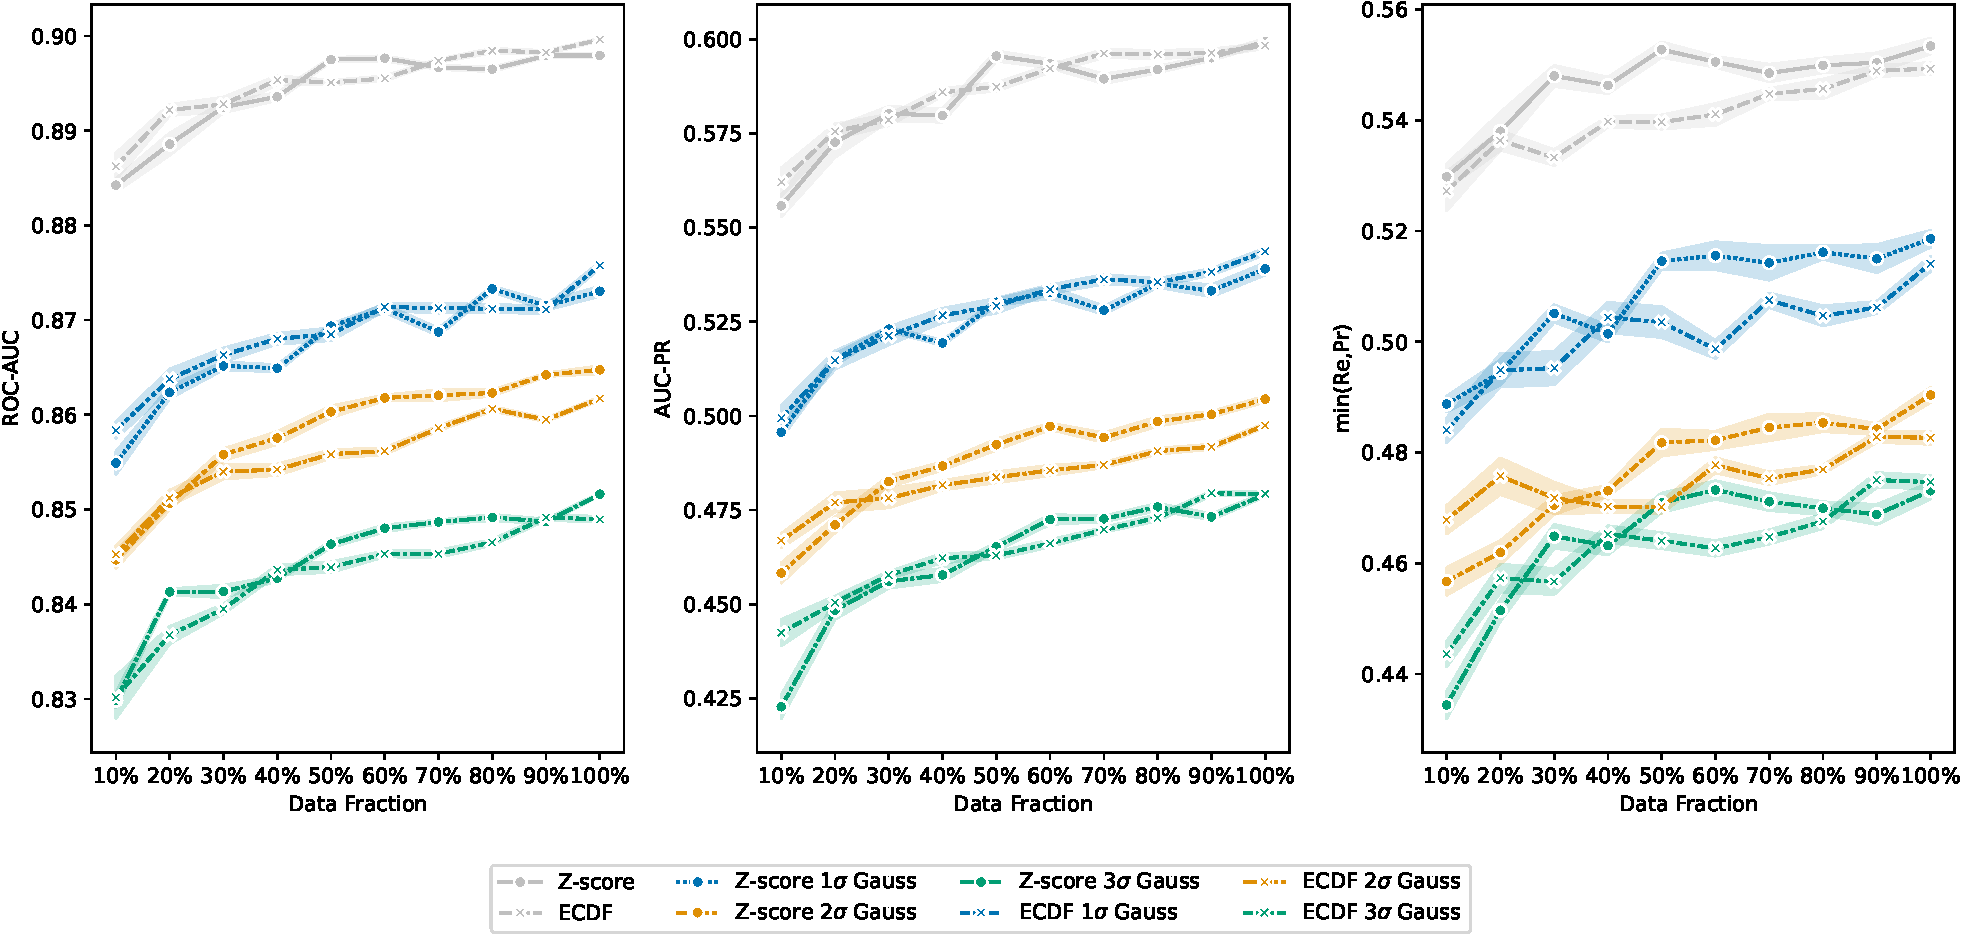
\includegraphics[width=\textwidth]{./figures/gaussian_noise_results}
    \caption{Comparison of performance metrics for mortality prediction under Gaussian noise across varying data fractions. X markers represent \gls{ecdf} normalization, and circles represent Z-score normalization. Lines of the same color correspond to the same noise level.}
    \label{fig:gaussian_noise_results}
\end{figure}


In experiments with Gaussian noise, there was no observable advantage in using \gls{ecdf} normalization over Z-score normalization. Both models, denoted by X markers for \gls{ecdf} and circles for Z-score in \cref{fig:gaussian_noise_results}, show similar performance across all data fractions and noise levels, with overlapping curves indicating similar results for each metric. As expected, increasing the noise level leads to an equivalent decrease in performance for both normalization approaches.

At the highest Gaussian noise level with the full dataset (\qty{100}{\percent} data fraction), model performance, as measured by \gls{auroc}, \gls{aucpr} and \gls{minrp}, dropped by \qty{5}{\percent} \qty{20}{\percent} and \qty{14}{\percent}, respectively, for both normalizations. Detailed results are provided in \cref{tab:noise_experiments}.



\subsection{Uniform Noise}
\label{sec:uniform_noise}

\begin{figure}
    \centering
    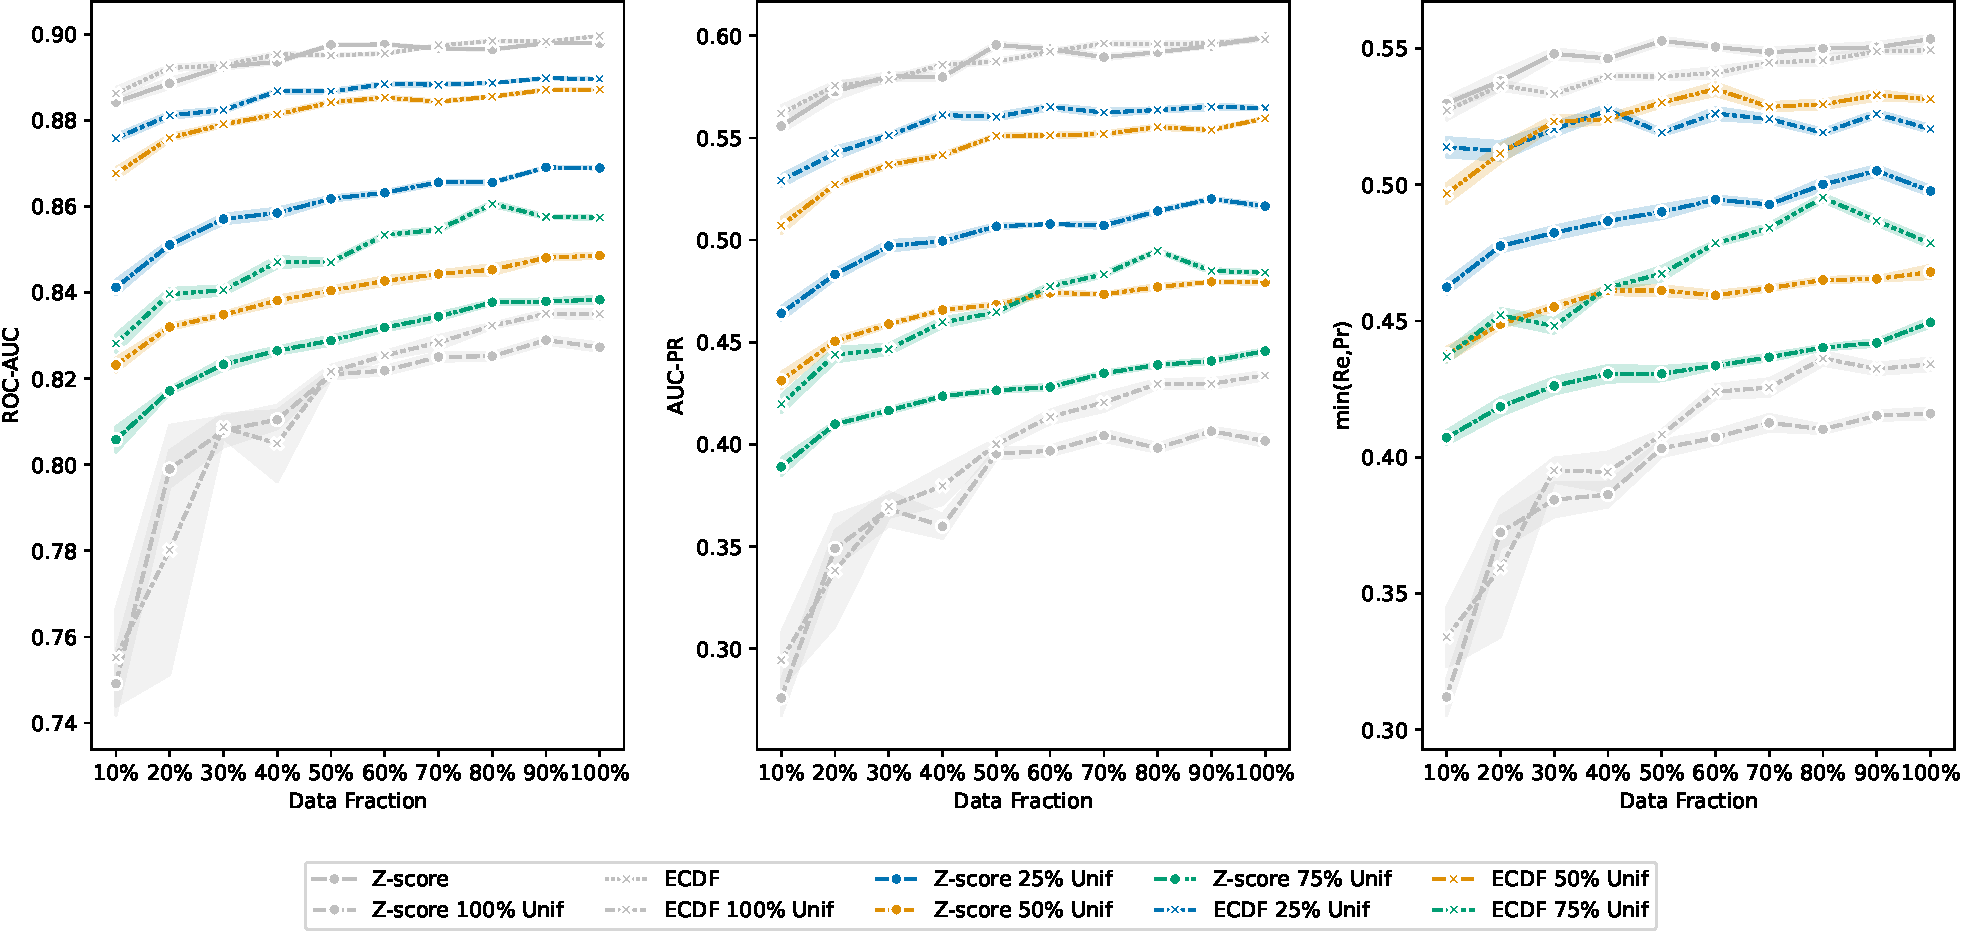
\includegraphics[width=\textwidth]{./figures/uniform_noise_results}
    \caption{Comparison of performance metrics for mortality prediction under uniform noise across varying data fractions. X markers represent \gls{ecdf} normalization, and circles represent Z-score normalization. Lines of the same color correspond to the same noise level.}
    \label{fig:uniform_noise_results}
\end{figure}


In contrast, the results with uniform noise show a clear advantage of \gls{ecdf} normalization in the presence of significant outliers introduced by the broad range of random values. Across all metrics, the performance of the \gls{ecdf}-normalized model consistently outperformed the Z-score normalized model, as indicated in \cref{fig:uniform_noise_results}.

Specifically, with the full dataset and \qty{75}{\percent} uniform noise, predictive performance metrics for Z-score normalization dropped by \qty{7}{\percent} for \gls{auroc}, \qty{26}{\percent} for \gls{aucpr}, and \qty{19}{\percent} for \gls{minrp} relative to noise-free data. In contrast, \gls{ecdf} normalization resulted in smaller reductions in performance, with declines of only \qty{4}{\percent}, \qty{18}{\percent}, and \qty{12}{\percent}, respectively. This suggests that \gls{ecdf} normalization provides greater resilience to extreme noise levels with a large number of outliers. We also observe that in the case of \qty{100}{\percent} noise, both normalization methods demonstrate similar performance, with intersecting error bands. This outcome aligns with our theoretical expectations discussed in \cref{sec:100_noise}.

However, directly comparing \gls{auroc} by percentage change can be misleading because the minimal reasonable performance starts from \(0.5\), representing random guessing. This limits the meaningful range for comparison and can exaggerate the perceived impact of changes. Furthermore, factors such as the model architecture's intrinsic robustness to outliers and the influence of demographic data, which were not affected by the added noise, can overshadow the effects of noise on other variables. For instance, the fusion attention module can inherently mitigate the influence of outliers by assigning them lower attention scores (see \cref{sec:fusion_self_attention}).


To more objectively analyze the effect of the normalization methods while minimizing the influence of these confounding factors, we propose reframing the analysis by examining how much of the model performance is retained relative to the extremes of completely noise-free data and entirely noisy data. We apply Min-Max scaling to the performance metrics, normalizing the results between the lowest achieved performance (average of experiments with complete noise) and the highest (average of experiments with pure data). We refer to these rescaled metrics as \textit{retained} predictive performance, where \qty{100}{\percent} represents the model's performance on noise-free data, and \qty{0}{\percent} represents performance when all observations are replaced with noise.


It is important to note that the analysis presented here may not adhere strictly to conventional statistical methodologies and may not be fully rigorous from a mathematical standpoint. Rather, it offers a new perspective aimed at isolating and comparing the effects of normalization methods independently of other factors influencing the model performance, providing insight into the specific impact of \gls{ecdf} and Z-score normalization on noise resilience.


\begin{table}
\begin{tabular}{p{1cm}p{1.2cm}ccc}
\toprule
Noise level &  & $\overline{\text{ROC-AUC}}$ \textuparrow & $\overline{\text{AUC-PR}}$ \textuparrow & $\overline{\text{min(Re,Pr)}}$ \textuparrow  \\
\midrule
 & \underline{Z-score} & 0.575\(\pm\)0.004 & 0.568\(\pm\)0.006 & 0.593\(\pm\)0.013 \\
\multirow[t]{2}{*}{25.0\%} & ECDF & \textbf{0.869\(\pm\)0.003 \(+51\%\)} & \textbf{0.820\(\pm\)0.004 \(+44\%\)} & \textbf{0.765\(\pm\)0.010 \(+29\%\)} \\
\cline{1-5}
 & \underline{Z-score} & 0.285\(\pm\)0.009 & 0.372\(\pm\)0.007 & 0.368\(\pm\)0.019 \\
\multirow[t]{2}{*}{50.0\%} & ECDF & \textbf{0.834\(\pm\)0.002 \(+193\%\)} & \textbf{0.794\(\pm\)0.003 \(+113\%\)} & \textbf{0.848\(\pm\)0.006 \(+130\%\)} \\
\cline{1-5}
 & \underline{Z-score} & 0.139\(\pm\)0.011 & 0.196\(\pm\)0.006 & 0.228\(\pm\)0.013 \\
\multirow[t]{2}{*}{75.0\%} & ECDF & \textbf{0.411\(\pm\)0.006 \(+196\%\)} & \textbf{0.397\(\pm\)0.004 \(+103\%\)} & \textbf{0.447\(\pm\)0.012 \(+96\%\)} \\
\cline{1-5}
\bottomrule
\end{tabular}

\caption{Retained mortality prediction performance on different metrics under uniform noise with \qty{100}{\percent} data fraction.}
\label{tab:noise_experiments_rescaled}
\end{table}

The results in \cref{tab:noise_experiments_rescaled} illustrate that \gls{ecdf} normalization substantially enhances resilience to uniform noise across all levels. Notably, under \qty{50}{\percent} noise, \gls{ecdf} normalization outperforms Z-score normalization demonstrating \qty{193}{\percent} higher retained \gls{auroc} and \qty{130}{\percent} higher retained \gls{minrp}.

Another noticeable trend is the relationship between the fraction of added noise and the retained performance. \gls{ecdf} normalization demonstrates a less-than-proportional decrease in performance as noise increases. For example, with a \qty{50}{\percent} noise level, the retained \gls{auroc}, \gls{aucpr}, and \gls{minrp} for \gls{ecdf} normalization are \qty{83}{\percent}, \qty{79}{\percent}, and \qty{85}{\percent}, respectively. This indicates that \gls{ecdf} normalization effectively mitigates the impact of noise. In contrast, Z-score normalization shows a greater-than-proportional decrease in performance under the same noise level, specifically \qty{29}{\percent}, \qty{37}{\percent}, and \qty{37}{\percent}, respectively. In fact, the retained performance of Z-score normalization drops nearly by half at just \qty{25}{\percent} noise level.

This trend persists even as noise levels increase. Under \qty{75}{\percent} noise, \gls{ecdf} normalization retains nearly triple the \gls{auroc} retention compared to Z-score normalization, and nearly double the retention of \gls{aucpr} and \gls{minrp}. These findings emphasize \gls{ecdf} normalization's robustness, particularly in handling high levels of noise and outliers, where it consistently sustains predictive performance.


\section{Chapter Conclusion}

In this chapter, we evaluated the performance of various experimental settings in the mortality prediction and time series forecasting, focusing on class balancing strategies, data normalization techniques, and robustness to noise. The \citefield{STraTS2022}{shorttitle} model, with implementation improvements, demonstrated superior performance, confirming its suitability as the foundation for further experimentation.

The introduction of \gls{ecdf} normalization showed promising results, especially in handling percentile-based predictions. This approach provided comparable fine-tuning performance metrics to Z-score normalization, though with enhanced resilience under uniform noise, which produced significant outliers. \gls{ecdf} normalization maintained predictive stability, underscoring its potential in applications with high variance or extreme values.

These results set the stage for an in-depth discussion on the implications of our findings. The next chapter will discuss the impact of observed results, their clinical relevance, and practical application.
